\documentclass{standalone}

\usepackage{pgfplots}

\pgfplotsset{compat=1.10}

\usepgfplotslibrary{fillbetween}

\begin{document}
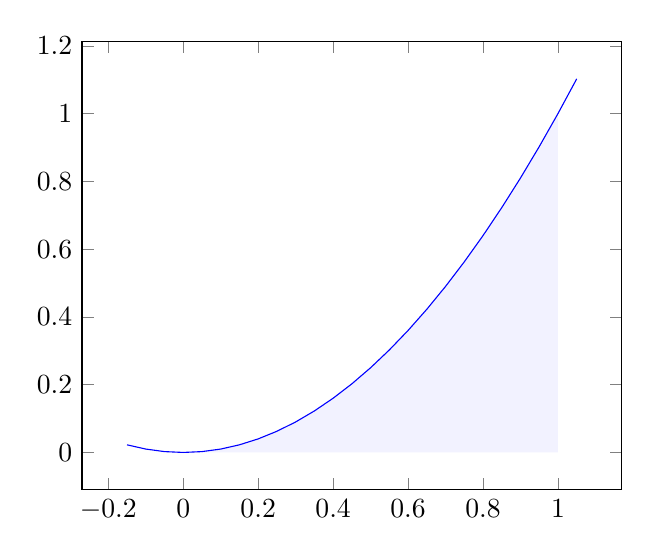
\begin{tikzpicture} 
    \begin{axis}[enlargelimits=0.1]
    \addplot[name path=f,domain=-.15:1.05,blue] {x^2};

 % scale=1,domain=0:90,samples=100,smooth,variable=\t]
 %      plot({-1*cos(\t)^(3)-13.5},{1*sin(\t)^(3)});

    \path[name path=axis] (axis cs:0,0) -- (axis cs:1,0);



    \addplot [
        thick,
        color=blue,
        fill=blue, 
        fill opacity=0.05
    ]
    fill between[
        of=f and axis,
        soft clip={domain=0:1},
    ];

    % \node [rotate=48] at (axis cs:  .7,  .59) {$y=x^2$};
    % \node [rotate=90] at (axis cs:  1.05,  .25) {$x=1$};
    \end{axis}
\end{tikzpicture}  
\end{document}